\begin{figure}[htbp]
\centering
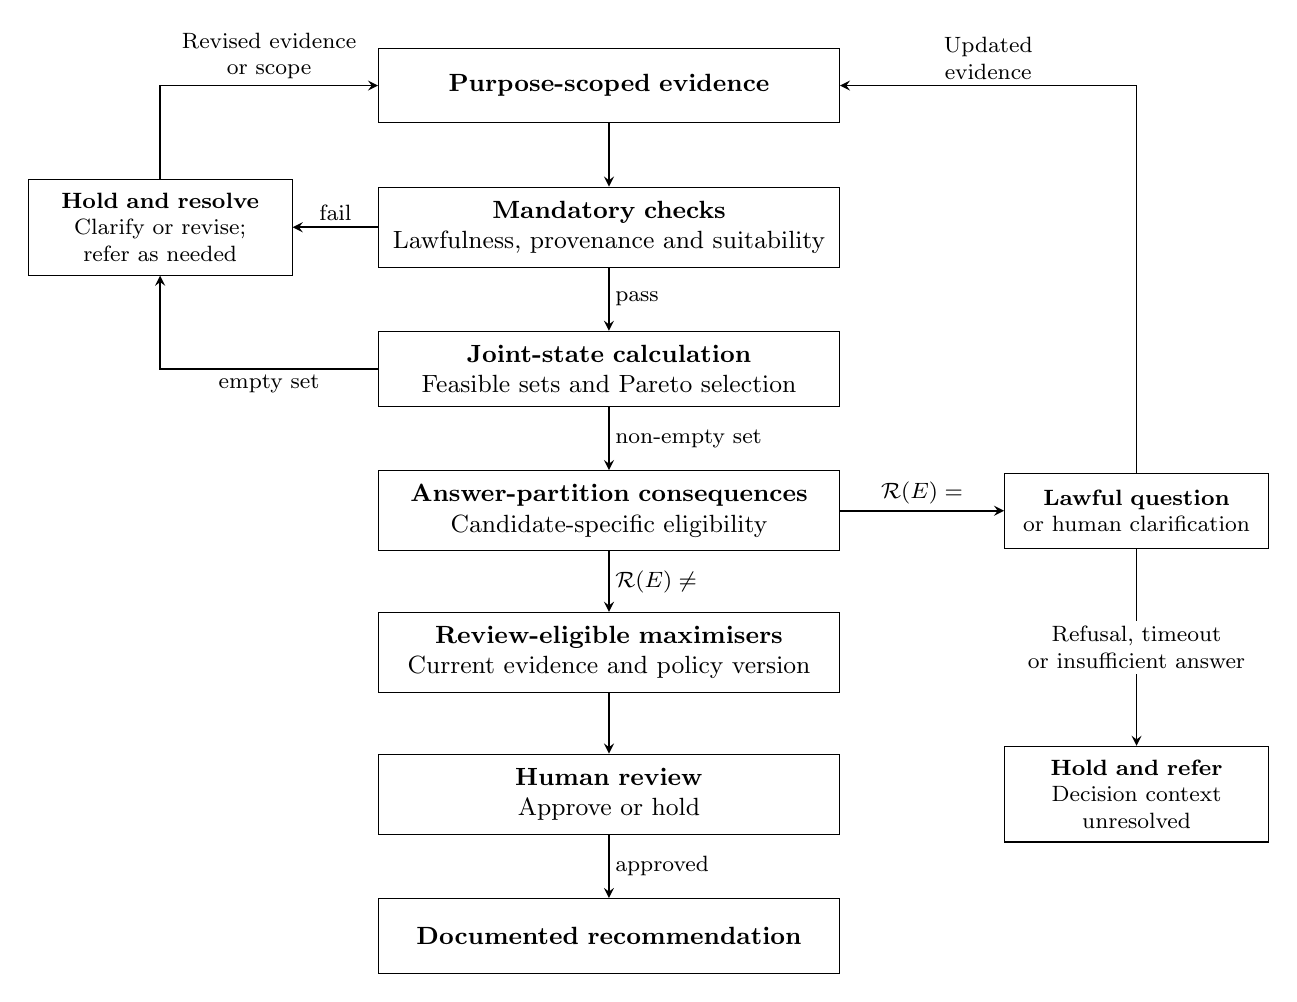
\begin{tikzpicture}[
  box/.style={draw, text width=5.5cm, minimum height=0.95cm,
    align=center, font=\small, inner sep=5pt},
  side/.style={draw, text width=3.0cm, minimum height=0.95cm,
    align=center, font=\footnotesize, inner sep=5pt},
  conn/.style={->, >=stealth, semithick},
  edge/.style={font=\footnotesize, fill=white, inner sep=2pt},
]
\node[box] (evidence) at (0,0) {\textbf{Purpose-scoped evidence}};
\node[box] (gates) at (0,-1.8)
  {\textbf{Mandatory checks}\\Lawfulness, provenance and suitability};
\node[box] (context) at (0,-3.6)
  {\textbf{Joint-state calculation}\\Feasible sets and Pareto selection};
\node[box] (facets) at (0,-5.4)
  {\textbf{Answer-partition consequences}\\Candidate-specific eligibility};
\node[box] (nash) at (0,-7.2)
  {\textbf{Review-eligible maximisers}\\Current evidence and policy version};
\node[box] (human) at (0,-9.0)
  {\textbf{Human review}\\Approve or hold};
\node[box] (advice) at (0,-10.8) {\textbf{Documented recommendation}};

\draw[conn] (evidence.south) -- (gates.north);
\draw[conn] (gates.south) -- node[edge,right] {pass} (context.north);
\draw[conn] (context.south) -- node[edge,right] {non-empty set} (facets.north);
\draw[conn] (facets.south) -- node[edge,right] {$\mathcal R(E)\ne\varnothing$} (nash.north);
\draw[conn] (nash.south) -- (human.north);
\draw[conn] (human.south) -- node[edge,right] {approved} (advice.north);

\node[side] (gatehold) at (-5.7,-1.8)
  {\textbf{Hold and resolve}\\Clarify or revise;\\refer as needed};
\draw[conn] (gates.west) -- node[edge,above] {fail} (gatehold.east);
\draw[conn] (gatehold.north) -- (-5.7,0)
  -- node[edge,above,align=center] {Revised evidence\\or scope} (evidence.west);
\draw[conn] (context.west) -- node[edge,below] {empty set}
  (-5.7,-3.6) -- (gatehold.south);

\node[side] (question) at (6.7,-5.4)
  {\textbf{Lawful question}\\or human clarification};
\draw[conn] (facets.east) -- node[edge,above] {$\mathcal R(E)=\varnothing$} (question.west);
\draw[conn] (question.north) -- (6.7,0)
  -- node[edge,above,align=center] {Updated\\evidence} (evidence.east);

\node[side] (contexthold) at (6.7,-9.0)
  {\textbf{Hold and refer}\\Decision context\\unresolved};
\draw[conn] (question.south) --
  node[edge,align=center] {Refusal, timeout\\or insufficient answer}
  (contexthold.north);
\end{tikzpicture}
\caption{Evidence-dependent calculation and version-bound approval in the restricted client selector.}
\label{fig:recommendation-flow}
{\raggedright\fignote{$\mathcal R(E)$ is the set of review-eligible maximisers at evidence state $E$. Approval binds a candidate to the current evidence and policy version. Source: the authors' recommendation procedure.}}
\end{figure}
